\documentclass[11pt,a4paper]{article}
\usepackage[utf8]{inputenc}
\usepackage[T1]{fontenc}
\usepackage[pt-BR]{babel}
\usepackage{graphicx}
\usepackage{float}
\usepackage{booktabs}
\usepackage{geometry}
\geometry{a4paper, margin=1in}
\usepackage{listings}
\usepackage{xcolor}
\usepackage{multicol}

% Configurações para blocos de código
\lstset{
    backgroundcolor=\color{gray!10},
    basicstyle=\ttfamily\small,
    frame=single,
    breaklines=true,
    captionpos=b,
    numbers=none
}

\title{Trabalho 1: Especificação - Parte 1}
\author{REDUX-V Arquitetura - Processador Mono-ciclo}
\date{}

\begin{document}

\maketitle

\section{Escolha de Instruções}
A arquitetura foi expandida para incluir as 3 instruções exigidas, sendo uma da lista pré-definida e duas inteiramente novas, elaboradas para facilitar construtos de iteração e cálculos com contadores.

\begin{table}[H]
\centering
\begin{tabular}{lllcl}
\toprule
\textbf{Tipo} & \textbf{Mnemonic} & \textbf{Nome} & \textbf{Opcode} & \textbf{Operação} \\
\midrule
R & inc & Increment & 0101 & R[ra] = R[rb] + 1 \\
R & dec & Decrement & 0110 & R[ra] = R[rb] - 1 \\
I & jnz & Jump Not Zero & 0111 & if (R[0] != 0) PC = PC + Imm (c/ sinal) \\
\bottomrule
\end{tabular}
\end{table}

\subsection*{Justificativa das Escolhas e Propostas}
A escolha estruturada dessas três instruções visa transformar a arquitetura fundamental em um processador altamente hábil para a execução de laços de repetição (loops) e varreduras de arrays (como manipulação de vetores de dados):
\begin{itemize}
    \item \textbf{inc (Increment)}: Escolhida da lista oficial. Avançar ponteiros e contadores é a rotina mais comum na computação em arrays. Ter uma instrução de uma via que realiza \texttt{R[ra] = R[rb] + 1} exclui a necessidade imperativa de devotar o registrador Acumulador (\texttt{R0}) injetando o imediato +1 via \texttt{addi 1} dentro do loop. Assim liberamos a pressão do uso exclusivo de \texttt{R0}.
    \item \textbf{dec (Decrement)}: Proposta nova. É o complemento simétrico ao \texttt{inc}. Com lexa, fica trivial fazer loops baseados em "contagem regressiva" até 0, uma técnica clássica para evitar testes de limite superior em código de montagem. Permite decrementar qualquer registrador ou o próprio contador de estado sem sujar o \texttt{R0} em etapas desnecessárias.
    \item \textbf{jnz (Jump Not Zero)}: Proposta nova. Na arquitetura original do REDUX-V, havia apenas o \texttt{brzr} (branch se for zero) que exige que o endereço-alvo do salto esteja rigidamente cravado em um registrador constante \texttt{R[rb]}. Isso queima um registrador precioso no minúsculo banco de dados (de 4 registradores apenas). A \texttt{jnz} é do Tipo I (com offset Imediato condicional). Se \texttt{R[0]} não zerou, o processador simplesmente soma o Imediato da instrução ao PC atual (\texttt{PC = PC + Imm}) e salta para o topo do loop de forma relativa, resolvendo toda a logística de repetição em apenas 1 instrução.
\end{itemize}

\newpage

\section{Algoritmos Implementados}

\subsection{1º Algoritmo Base}
O algoritmo itera sobre \texttt{i} (0 até a-1). Substituímos o teste abstrato por um \texttt{counter} em R[0] que decresce de \texttt{a} (3) até 0; iteramos o valor (b+i) em R[1] e o endereço M[c+i] em R[2]. Usamos a instrução \texttt{jnz} para simplificar o loop branchless e poupar registradores.

\subsubsection*{Estratégia de Construção de Constantes Grandes (Shift-Add)}
Como determinam as regras estruturais da arquitetura original do REDUX-V, a única porta de entrada para puxar constantes nativamente "direto do papel" (os Imediatos) e ejetá-los para dentro dos registradores é por meio da instrução \texttt{addi}. Contudo, o Imediato inserido pelo próprio formato do opcode é travado em um espaço de instrução de meros \textbf{4-bits com sinal}, cujo valor máximo transferido é travado em \textbf{+7}.

Para carregar um número grande como escalar \texttt{b = 42} ou o ponteiro \texttt{c = 10}, o \textit{setup} levaria diversas rodadas infáveis do processador somando o máximo número natural  (\texttt{addi 7}). Para contornar e otimizar a criação desse número elevado e seguir respeitando rigorosamente o limite de instruções do processador REDUX-V, implementei a clássica técnica e ginástica de \textit{Shift-Add}:
\begin{itemize}
    \item Lança-se primeiro um número "raiz / semente" primário que cabe no Imediato de tamanho reduzido, por exemplo \texttt{addi 5}.
    \item Usamos uma instrução base e barata de \texttt{add R0, R0} de somar o registrador consigo próprio. O resultado é o infalível efeito aritmético multiplicativo (fator de *Shift-Left*, vezes 2). Imediatamente a semente \texttt{5} vira \texttt{10}. Ao encadear os dobros, a contagem atinge a grandeza desejada exponencialmente: \texttt{10 -> 20 -> 40}.
    \item Finaliza-se preenchendo o saldo (\textit{offset}) através de um mergulho fracionado final do resto da divisão modular. Neste caso \texttt{addi 2}.
\end{itemize}
Pronto! Com apenas um saldo primário e punhado enxuto de saltos, injetamos diretamente do hardware o valor limpo, total num piscar enxugado em 5 instruções precisas aos registros sem macular nenhuma linha estrutural nem depender da memória RAM paralela.

\vspace{0.5cm}
\begin{multicols}{2}
\textbf{Linguagem C / Lógica}
\begin{lstlisting}[language=C]
int i;
int a = 3;
int b = 42;
int *c = 10;
for (i = 0; i < a; i++) {
  c[i] = b + i;
}
\end{lstlisting}

\columnbreak

\textbf{Mapeamento Registradores}
\begin{lstlisting}
R0 = Counter / Accum
R1 = Val (b+i, começa em 42)
R2 = Ptr (c+i, começa em 10)
\end{lstlisting}
\end{multicols}

\textbf{Assembly REDUX-V}
\begin{lstlisting}
# 1. Carregar Val (R1) = 42
sub R0, R0      # R0 = 0
addi 5          # R0 = 5
add R0, R0      # R0 = 10
add R0, R0      # R0 = 20
add R0, R0      # R0 = 40
addi 2          # R0 = 42
sub R1, R1      # R1 = 0
add R1, R0      # R1 = 42

# 2. Carregar Ptr (R2) = 10
sub R0, R0      # R0 = 0
addi 5          # R0 = 5
add R0, R0      # R0 = 10
sub R2, R2      # R2 = 0
add R2, R0      # R2 = 10

# 3. Inicializar Loop Counter (R0) = a = 3
sub R0, R0      # R0 = 0
addi 3          # R0 = 3

loop_start:
st R1, R2       # M[R2] = R1  (c[i] = b+i)
inc R1, R1      # Val++       (prox. valor)
inc R2, R2      # Ptr++       (prox. end.)
dec R0, R0      # Counter--
jnz -4          # se R0 != 0, salta para loop_start
\end{lstlisting}

\textbf{Código de Máquina (Binário puro - Hexadecimal)}
\begin{table}[H]
\centering
\begin{tabular}{clccl}
\toprule
\textbf{Memória} & \textbf{Assembly} & \textbf{Hex} & \textbf{Binário} & \textbf{Anotação} \\
\midrule
0x00 & sub R0, R0 & D0 & 1101 0000 & Ra=0, Rb=0 \\
0x01 & addi 5     & 45 & 0100 0101 & \\
0x02 & add R0, R0 & C0 & 1100 0000 & \\
0x03 & add R0, R0 & C0 & 1100 0000 & \\
0x04 & add R0, R0 & C0 & 1100 0000 & \\
0x05 & addi 2     & 42 & 0100 0010 & R0 = 42 \\
0x06 & sub R1, R1 & D5 & 1101 0101 & Ra=1, Rb=1 \\
0x07 & add R1, R0 & C4 & 1100 0100 & Ra=1, Rb=0 \\
0x08 & sub R0, R0 & D0 & 1101 0000 & \\
0x09 & addi 5     & 45 & 0100 0101 & \\
0x0A & add R0, R0 & C0 & 1100 0000 & R0 = 10 \\
0x0B & sub R2, R2 & DA & 1101 1010 & Ra=2, Rb=2 \\
0x0C & add R2, R0 & C8 & 1100 1000 & Ra=2, Rb=0 \\
0x0D & sub R0, R0 & D0 & 1101 0000 & \\
0x0E & addi 3     & 43 & 0100 0011 & R0 = 3 \\
0x0F & st R1, R2  & 36 & 0011 0110 & Ra=1, Rb=2 \\
0x10 & inc R1, R1 & 55 & 0101 0101 & Ra=1, Rb=1 \\
0x11 & inc R2, R2 & 5A & 0101 1010 & Ra=2, Rb=2 \\
0x12 & dec R0, R0 & 60 & 0110 0000 & Ra=0, Rb=0 \\
0x13 & jnz -4     & 7C & 0111 1100 & -4 = 1100 (c2) \\
\bottomrule
\end{tabular}
\end{table}

\newpage

\subsection{2º Algoritmo Customizado (Memcpy)}
O algoritmo de Cópia de Memória (\textit{Memory Copy}) demonstra a força do design de instruções conjuntas \texttt{inc}, \texttt{dec} e \texttt{jnz}. Ele é encarregado de copiar um bloco de dados de modo contínuo na arquitetura, lendo do endereço inicial origem (p.ex. a posição 20) e gravando para o endereço destino (p.ex. a posição 40). O bloco copiará sequencialmente 10 posições de memória.

\textbf{Setup dos Registradores (Inicialização)}
\begin{itemize}
    \item \texttt{R1 = 20} (Ponteiro de Origem - \textit{Source Pointer})
    \item \texttt{R2 = 40} (Ponteiro de Destino - \textit{Dest Pointer})
    \item \texttt{R0 = 10} (Contador do laço de repetição)
    \item \texttt{R3 = Usado como a variável temporária do dado em trânsito} 
\end{itemize}

O código em Assembly fica elegantemente condensado em exatamente 6 instruções para compor o laço (motor da cópia):
\begin{lstlisting}
... (setup dos registradores via rotinas addi repetidas foram omitidos para foco no laco) ...

loop:
ld R3, R1     #(1) Le dado na origem R1 e salva temporariamente em R3
st R3, R2     #(2) Grava dado flutuante em R3 no destino R2
inc R1, R1    #(3) Avanca o ponteiro de origem (+1 posicao)
inc R2, R2    #(4) Avanca o ponteiro de destino (+1 posicao)
dec R0, R0    #(5) Reduz o montante de vezes que ainda falta rodar
jnz -5        #(6) Repete enquanto R0 nao bateu valor nulo cravado
\end{lstlisting}


\vspace{0.5cm}
\textbf{Código de Máquina (Binário puro - Hexadecimal)}
\begin{table}[H]
\centering
\begin{tabular}{clccl}
\toprule
\textbf{Memória} & \textbf{Assembly} & \textbf{Hex} & \textbf{Binário} & \textbf{Anotação} \\
\midrule
0x20 & ld R3, R1  & 2D & 0010 1101 & Ra=11, Rb=01 \\
0x21 & st R3, R2  & 3E & 0011 1110 & Ra=11, Rb=10 \\
0x22 & inc R1, R1 & 55 & 0101 0101 & Ra=01, Rb=01 \\
0x23 & inc R2, R2 & 5A & 0101 1010 & Ra=10, Rb=10 \\
0x24 & dec R0, R0 & 60 & 0110 0000 & Ra=00, Rb=00 \\
0x25 & jnz -5     & 7B & 0111 1011 & -5 = 1011 (c2) \\
\bottomrule
\end{tabular}
\end{table}
\vspace{0.2cm}

\subsubsection*{Cálculo e Dinâmica do Pulo: Por que "-5"?}
A operação condicional que repete o loop, \texttt{jnz -5}, está alocada ancorada no endereço de hardware \texttt{0x25}. O comportamento de um Desvio Relativo ao PC leva em conta pela regra matemática a fórmula de salto: \texttt{PC = PC + Imediato}. 

Pela definição unívoca do nosso diagrama de hardware do processador (*Datapath* visualizado a seguir), o \textit{Adder} para deslocamento está interligado extraindo os dados diretamente da saída inicial do \texttt{PC local} que indexou a ação.

A lógica resolvida temporalmente no hardware dita:
\begin{center}
\texttt{PC\_Alvo = PC\_Atual + Imediato} \\
\texttt{PC\_Alvo = 0x25 + (-5)} \\
\textbf{\texttt{PC\_Alvo = 0x20}}
\end{center}

Portanto, o salto direciona estritamente o cursor de volta à exata chave local \texttt{0x20}, que assenta com perfeição mecânica de volta ao topo do bloco do loop para ler o novo pacote de dados: \texttt{ld R3, R1}. 

\newpage

\section{Diagramas e Sinais de Controle}

\subsection{Diagrama do Caminho de Dados (Datapath)}
\begin{figure}[hbtp]
    \centering
    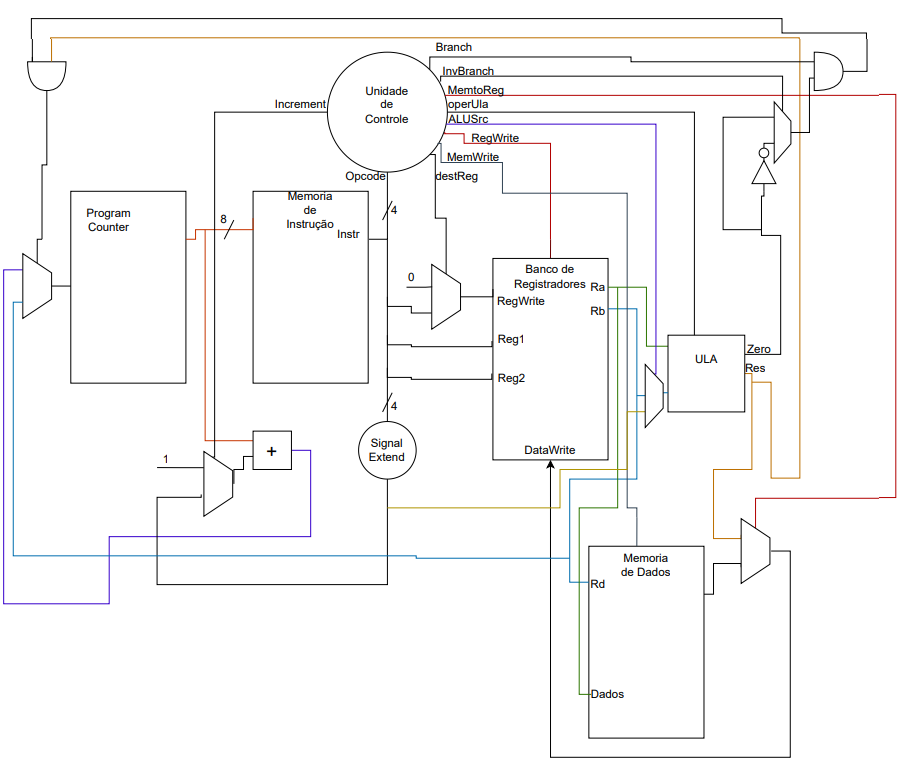
\includegraphics[width=0.75\linewidth]{Datapath.png}
    \caption{Datapath do ReduxV}
    \label{fig:datapath}
\end{figure}

\subsection{Diagrama Interno da ULA (ALU)}
\begin{figure}[hbtp]
    \centering
    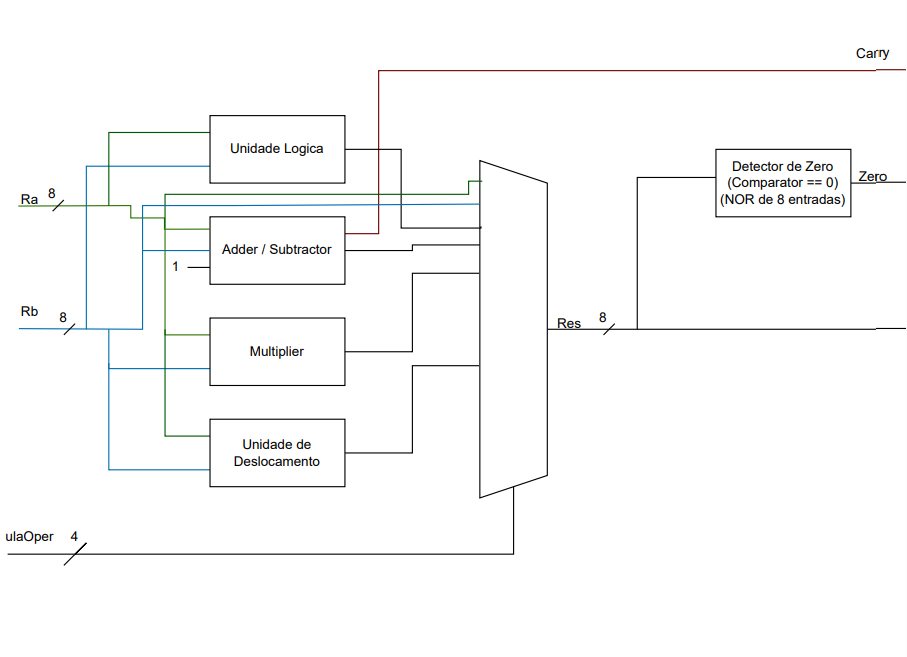
\includegraphics{diagramaUla.png}
    \caption{Diagrama da ULA}
    \label{fig:ula}
\end{figure}

\newpage

\subsection{Tabela de Sinais de Controle}
\begin{table}[H]
\centering
\resizebox{\textwidth}{!}{
\begin{tabular}{lccccccccc}
\toprule
\textbf{Inst./Opcode} & \textbf{Increment} & \textbf{Branch} & \textbf{InvBranch} & \textbf{MemToReg} & \textbf{ULAsrc} & \textbf{RegWrite} & \textbf{MemRight} & \textbf{destReg} & \textbf{operULA}
\midrule
brzr (0000) & 0 & 1 & 0 & 0 & 0 & 0 & 0 & 0 & -- \\
ji (0001)   & 0 & 1 & 0 & 0 & 0 & 0 & 0 & 0 & -- \\
ld (0010)   & 0 & 0 & 0 & 1 & 0 & 1 & 0 & 0 & -- \\
st (0011)   & 0 & 0 & 0 & 0 & 0 & 0 & 1 & 0 & -- \\
addi (0100) & 0 & 0 & 0 & 0 & 1 & 1 & 0 & 0 & add \\
inc (0101)  & 1 & 0 & 0 & 0 & 1 & 1 & 0 & 0 & add \\
dec (0110)  & 1 & 0 & 0 & 0 & 1 & 1 & 0 & 0 & sub \\
jnz (0111)  & 0 & 1 & 1 & 0 & 0 & 0 & 0 & 0 & -- \\
not (1000)  & 0 & 0 & 0 & 0 & 0 & 1 & 0 & 0 & not \\
and (1001)  & 0 & 0 & 0 & 0 & 0 & 1 & 0 & 0 & and \\
or (1010)   & 0 & 0 & 0 & 0 & 0 & 1 & 0 & 0 & or  \\
xor (1011)  & 0 & 0 & 0 & 0 & 0 & 1 & 0 & 0 & xor \\
add (1100)  & 0 & 0 & 0 & 0 & 0 & 1 & 0 & 0 & add \\
sub (1101)  & 0 & 0 & 0 & 0 & 0 & 1 & 0 & 0 & sub \\
slr (1110)  & 0 & 0 & 0 & 0 & 0 & 1 & 0 & 0 & slr \\
srr (1111)  & 0 & 0 & 0 & 0 & 0 & 1 & 0 & 0 & srr \\
\bottomrule
\end{tabular}
}
\end{table}

\end{document}
